\documentclass{article}%
\usepackage[T1]{fontenc}%
\usepackage[utf8]{inputenc}%
\usepackage{lmodern}%
\usepackage{booktabs}%
\usepackage{textcomp}%
\usepackage{lastpage}%
\usepackage{geometry}%
\usepackage{amsmath}%
\geometry{
    paper=a4paper,
    head=0cm,
    left=2cm,
    right=2cm,
    top=0cm,
    bottom=2cm,
    includehead=True,
    includefoot=True
}%
\usepackage{graphicx}%
%
\usepackage{multicol}%
\usepackage{lipsum}%
\usepackage{float}%
\usepackage{verbatim}%
\title{
    Reconstructing Arrival-Times of individual Photons
    in a continous Stream of Night-Sky-Light
}%
\author{Sebastian A. Mueller}%
\date{}%
%
\begin{document}%
\maketitle%

\newcommand{\F}{F_\text{night-sky-background}}
\newcommand{\Ftyp}{F_\text{dark-night}}
\begin{multicols}{2}%
%
The atmospheric Cherenkov-method can reconstruct the type, energy, and direction of a cosmic particle.
%
The reconstructions depend solely on the quality of the recorded Cherenkov-light-field.
%
\section*{Night-Sky-Background}%
\label{sec:nsb}%
%
Typical photo-sensors in the atmospheric-Cherenkov method yield night-sky-photon-rates of
\begin{eqnarray*}
R_\text{PMT} &=& 144.8\times10^6\,\text{m}^{-2}\,(1^\circ)^{-2}\,\text{s}^{-1}\\
R_\text{SiPM} &=& 280.3\times10^6\,\text{m}^{-2}\,(1^\circ)^{-2}\,\text{s}^{-1}.
\end{eqnarray*}
%
The rates result out of the typical flux $\F{}$ during observations, see Figure \ref{fig:nsb}, and the corresponding photon-detection-efficiencies, see Figure \ref{fig:pde}.
%
The typical flux  corresponds to a sky surface brightness of
%
\begin{eqnarray*}
\F{} &\hat{=}& 21\,\text{mag}\,\text{arcsec}^{-2}.
\end{eqnarray*}
%
Observations take place in the range of fluxes from
\begin{eqnarray*}
0.75 &> \F{} / \Ftyp{} >& 4.
\end{eqnarray*}
%
New moon, full moon, and clouds all impact $\F{}$.
%
Figure \ref{fig:obstimeFact} shows the flux distribution during observations with a Cherenkov-telescope which tried hard to observe in the brightest conditions using silicon photo-sensors which can tolerate this stress.
%
Table \ref{TabInstrumentsNsbRates} shows the expected rates of night-sky-photons in different instruments.
%
\begin{figure}[H]%
\centering%
\includegraphics[width=1.0\linewidth]{night_sky_background.jpg}%
\caption{
The typical flux $F_\text{Night}$ of night-sky-light \cite{benn1987night},
extrapolated from 700 - 1000\,nm. Dotted line is \cite{preuss2002study}.
}%
\label{fig:nsb}
\end{figure}
%
\begin{figure}[H]%
\centering%
\includegraphics[width=1.0\linewidth]{photon_efficiency.jpg}%
\caption{
Dotted line is silicon-photo-multiplier (SiPM) \cite{hamamatsu2009mppc},
Extrapolated from 700 - 1000\,nm.
Dashed line is photo-multiplier-tube (PMT) \cite{toyama2013novel}
}%
\label{fig:pde}
\end{figure}
%
\begin{figure}[H]%
\centering%
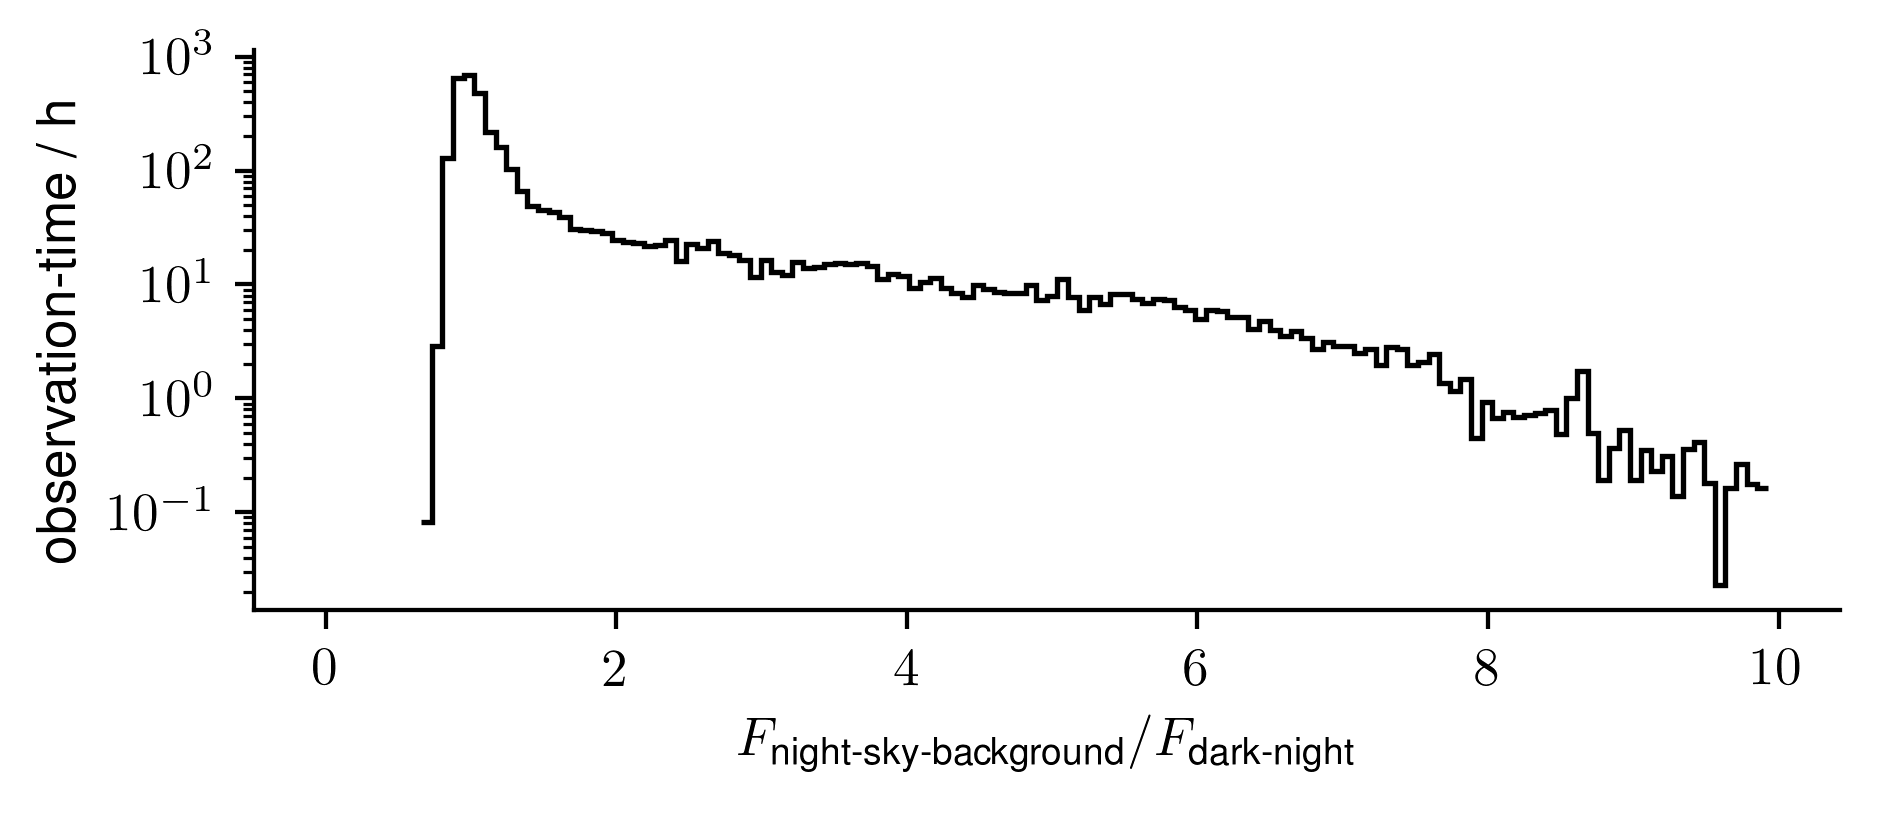
\includegraphics[width=1.0\linewidth]{observation_time_histogram.png}%
\caption{
The observations of FACT, taken from Sebastian's phd-thesis.
}%
\label{fig:obstimeFact}
\end{figure}
%
\begin{table}[H]
  \begin{center}
    \begin{tabular}{lcrrr}
        &tech.& area/ & fov/&$R$/\\
        &     & m$^2$ & $(1^\circ)^{2}$&$10^6$s$^{-1}$\\
      \hline
      FACT &SiPM& 10 & 0.01 & 29\\
      H.E.S.S. CT-1 &PMT& 108 & 0.0222 & 344\\
      H.E.S.S. CT-5 &PMT& 614 & 0.0039 & 347\\
      Portal, 71m &PMT& 65 & 0.0039 & 37\\
    \end{tabular}
    \caption{Expected rates of night-sky-photons $R$ in an individual read-out-channel (pixel or lixel).}
    \label{TabInstrumentsNsbRates}
  \end{center}
\end{table}
%
\bibliographystyle{apalike}%
\bibliography{/home/relleums/Desktop/starter_kit/sebastians_references/references}%
\end{multicols}{2}%
\end{document}
